% Generated by generar_informe.py for VP_20262509_1500_22QR_60_robots.csv. Manual remarks go in notas.tex.
\begingroup
% Generated by generar_informe.py -- do not edit; re-run the script instead.
\def\VTitulo{20262509\_1500\_22QR\_60}
\def\VArchivo{VP\_20262509\_1500\_22QR\_60\_robots.csv}
\def\VVideo{VC\_20262509\_1500\_22QR\_60.MP4}
\def\VFrameIni{0}
\def\VFrameFin{11011}
\def\VCuadros{11012}
\def\VFps{3}
\def\VDuracion{3.67e+03}
\def\VN{22}
\def\VUnidadL{cm}
\def\VUnidadV{mm/s}
\def\VEscala{0.3715}
\def\VEscalaFuente{escala exportada por la app (diámetro real cargado en la pestaña Seguimiento)}
\def\VEscalaQ{\SI{0.3715}{\milli\metre\per px}}
\def\VFpsQ{\num{3} cuadros = \SI{1}{\second} real ($\Delta t = \SI{0.333}{\second}$)}
\def\VDuracionQ{\SI{61.2}{\minute}}
\def\VRescala{tomada del CSV exportado}
\def\VDiamQ{\SI{35}{\milli\metre} $\equiv$ \SI{94.2}{px}}
\def\VUL{\centi\metre}
\def\VUV{\milli\metre\per\second}
\def\VDiamMM{35}
\def\VDiamPx{94.2}
\def\VPctObs{100}
\def\VPctRot{100}
\def\VNErr{0}
\def\VNAdv{0}
\def\VVmedia{1.1}
\def\VVmediana{0.697}
\def\VVpNoventaycinco{3.55}
\def\VRecMedio{486}
\def\VNetoMedio{10.9}

\section{Ensayo \VTitulo}\label{sec:20262509_1500_22QR_60}

\begin{table}[H]
  \centering
  \caption{Datos del ensayo \VTitulo.}
  \begin{tabular}{@{}lp{0.58\linewidth}@{}}
    \toprule
    Archivo de datos & \texttt{\VArchivo} \\
    Video & \texttt{\VVideo} \\
    Cuadros analizados & \VFrameIni\,--\,\VFrameFin{} (\num{\VCuadros}) \\
    Escala de tiempo & \VFpsQ\newline{\footnotesize\VRescala} \\
    Duración real & \VDuracionQ \\
    Robots seguidos ($N$) & \num{\VN} \\
    Diámetro del robot & \VDiamQ \\
    Escala & \VEscalaQ\newline{\footnotesize\VEscalaFuente} \\
    Origen de coordenadas & \VOrigen \\
    Recinto & \VRecinto \\
    Posiciones observadas & \SI{\VPctObs}{\percent} \\
    Cuadros con error / con advertencia & \num{\VNErr} / \num{\VNAdv} \\
    \bottomrule
  \end{tabular}
\end{table}

\IfFileExists{generado/20262509_1500_22QR_60/captura.png}{%
\begin{figure}[H]
  \centering
  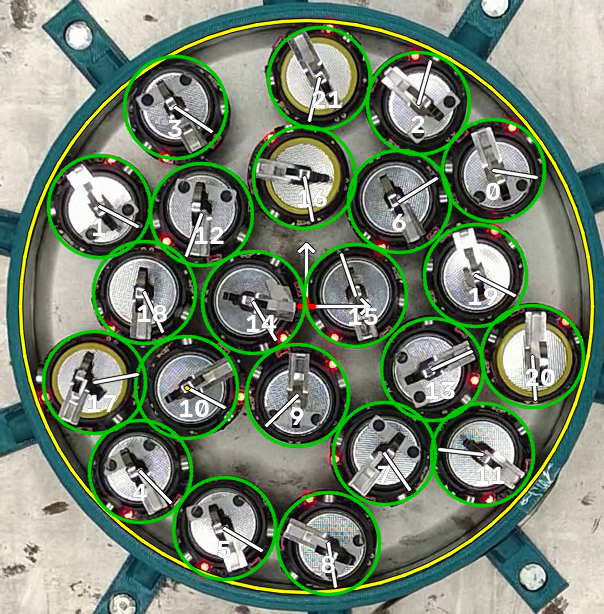
\includegraphics[width=0.62\linewidth]{generado/20262509_1500_22QR_60/captura.png}
  \caption{Cuadro de ejemplo con identificador, vector velocidad (amarillo, largo = desplazamiento en 7,5 cuadros) y orientación (aguja blanca). Círculo verde: posición observada; naranja: estimada. Imagen rotada 180° (vista del observador): $x$ a la derecha, $y$ hacia arriba (lejos del observador).}
\end{figure}}{}

\begin{figure}[H]
  \centering
  \begin{tikzpicture}
    \begin{axis}[width=0.97\linewidth, height=5.2cm, xlabel={$t$ [\si{\minute}]},
        ylabel={$|\vec v|$ [\si{\milli\metre\per\second}]}, ymin=0, grid=major, grid style={gray!20}, scaled ticks=false, tick label style={/pgf/number format/fixed, /pgf/number format/precision=3},
        legend pos=north east, legend style={font=\footnotesize}, enlarge x limits=false]
      \addplot [name path=q75, draw=none, forget plot] table [x=t, y=v_q75, col sep=comma] {generado/20262509_1500_22QR_60/serie.csv};
      \addplot [name path=q25, draw=none, forget plot] table [x=t, y=v_q25, col sep=comma] {generado/20262509_1500_22QR_60/serie.csv};
      \addplot [azul!25] fill between [of=q25 and q75];
      \addlegendentry{rango intercuartil}
      \addplot [azul, thick] table [x=t, y=v_mean, col sep=comma] {generado/20262509_1500_22QR_60/serie.csv};
      \addlegendentry{media de los $N$ robots}
    \end{axis}
  \end{tikzpicture}
  \caption{Rapidez de los robots en función del tiempo.}
\end{figure}

\begin{figure}[H]
  \centering
  \begin{tikzpicture}
    \begin{axis}[width=0.8\linewidth, height=5cm, xlabel={$|\vec v|$ [\si{\milli\metre\per\second}]},
        ylabel={densidad [\si{\second\per\milli\metre}]},
        ymin=0, enlarge x limits=false, grid=major, grid style={gray!20},
        scaled ticks=false, tick label style={/pgf/number format/fixed, /pgf/number format/precision=3}]
      \addplot [fill=azul!35, draw=azul, const plot mark left] table [x=v, y=dens, col sep=comma] {generado/20262509_1500_22QR_60/hist_v.csv} \closedcycle;
    \end{axis}
  \end{tikzpicture}
  \caption{Distribución de la rapidez (solo posiciones observadas).}
\end{figure}

\begin{figure}[H]
  \centering
  \begin{tikzpicture}
    \begin{axis}[width=0.72\linewidth, axis equal image, xlabel={$x$ [\si{\centi\metre}]},
        ylabel={$y$ [\si{\centi\metre}]}, grid=major, grid style={gray!20}, cycle list name=robots,
        tick label style={font=\footnotesize}]
      \pgfplotsinvokeforeach{0,...,21}{%
        \addplot+ [thin, no markers] table [x=x#1, y=y#1, col sep=comma] {generado/20262509_1500_22QR_60/tray.csv};}
      \draw [gray, thick] (axis cs:0,0) circle [radius=9.25];
      \addplot [only marks, mark=+, mark size=3pt, black] coordinates {(0,0)};
    \end{axis}
  \end{tikzpicture}
  \caption{Trayectorias de los 22 robots (imagen rotada 180° (vista del observador); origen en el centro del recinto, $y$ hacia arriba; círculo gris: pared interior), primeros 5 minutos reales.}
\end{figure}

\begin{figure}[H]
  \centering
  \begin{tikzpicture}
    \begin{axis}[width=0.97\linewidth, height=5.4cm, xlabel={$t$ [\si{\minute}]},
        ylabel={$\theta$ [vueltas]}, grid=major, grid style={gray!20}, cycle list name=robots, enlarge x limits=false]
      \pgfplotsinvokeforeach{0,...,21}{%
        \addplot+ [thin, no markers] table [x=t, y=th#1, col sep=comma] {generado/20262509_1500_22QR_60/theta.csv};}
    \end{axis}
  \end{tikzpicture}
  \caption{Orientación acumulada de cada robot ($\theta=0$ en el primer cuadro; positivo = antihorario).}
\end{figure}

\begin{table}[H]
  \centering
  \caption{Resumen por robot.}
  \footnotesize
  \pgfplotstabletypeset[col sep=comma, columns={id,obs,vmed,vmax,rec,net,vueltas,wabs},
      every head row/.style={before row=\toprule, after row=\midrule}, every last row/.style={after row=\bottomrule},
      columns/id/.style={column name={Robot}, int detect},
      columns/obs/.style={column name={Obs. [\si{\percent}]}, fixed, precision=1},
      columns/vmed/.style={fixed, fixed zerofill, precision=2, column name={$\overline{|\vec v|}$ [\si{\milli\metre\per\second}]}},
      columns/vmax/.style={fixed, fixed zerofill, precision=2, column name={$|\vec v|_{\max}$ [\si{\milli\metre\per\second}]}},
      columns/rec/.style={fixed, fixed zerofill, precision=2, column name={Recorrido [\si{\centi\metre}]}},
      columns/net/.style={fixed, fixed zerofill, precision=2, column name={Despl. neto [\si{\centi\metre}]}}, columns/vueltas/.style={column name={$\theta_{\mathrm{final}}$ [vueltas]}, fixed, precision=2},
      columns/wabs/.style={column name={$\overline{|\omega|}$ [\si{\degree\per\second}]}, fixed, fixed zerofill, precision=1},
    ]{generado/20262509_1500_22QR_60/resumen.csv}
\end{table}

\subsection{Lo observado}
Se siguieron \num{22} robots durante \num{11012} cuadros (\SI{61.2}{\minute}). El \SI{100}{\percent} de las posiciones fue observado (detectado o corregido a mano); el resto se estimó por interpolación o predicción.
No hubo cuadros con posiciones estimadas.
La rapidez mediana fue \SI{0.606}{\milli\metre\per\second} y el percentil 95, \SI{3.09}{\milli\metre\per\second}: la cola rápida es \num{5.1} veces la mediana, lo que indica movimiento intermitente, con episodios cortos de alta velocidad.
El robot más rápido en promedio fue el \num{3} (\SI{1.78}{\milli\metre\per\second}).
En rotación, \num{14} robots giraron en neto en sentido antihorario, \num{8} en sentido horario y \num{0} giraron menos de media vuelta. El que más giró fue el \num{3}, con $|\omega|$ media de \SI{23.6}{\degree\per\second}. La rotación se midió directamente en el \SI{100}{\percent} de los puntos.

\IfFileExists{generado/20262509_1500_22QR_60/notas.tex}{% Observaciones propias sobre este ensayo (este archivo no se sobrescribe).
% Ejemplo:
% \paragraph{Notas.} A partir de $t\approx\SI{3}{\second}$ los robots se
% agrupan contra la pared norte de la arena.
}{}
\endgroup
